\section{Situación Actual}

En la actualidad podemos encontrar diversos intentos de modernizar los procesos administrativos de entidades públicas y podemos tomar sus experiencias como inspiración para la realización de una herramienta reutilizable de software. Además, existen paquetes de software que, aunque de manera indirecta, pueden ayudar en la creación de trámites.

\subsection{Sistemas realizados para el control de trámites}

Sólo en Latinoamérica, cada país reportó mediante las autoridades de gobierno electrónico tener entre 1000 y 5000 trámites diferentes. Esto implica que ya hubo muchos esfuerzos para crear sistemas que digitalicen esta actividad. A continuación se listan algunos.

\subsubsection{A nivel académico}

Podemos encontrar una gran cantidad de proyectos de grado realizados en la región que tratan sobre la implementación de sistemas de control de trámites:

\begin{itemize}
    \item SISTEMA DE CONTROL DE TRÁMITES UTILIZANDO MAQUINAS DE TURING CASO: DIVISIÓN DE GESTIONES ADMISIONES Y REGISTROS U.M.S.A.
    \item Desarrollo e Implementación del Sistema de Tramite
          Documentario en la Municipalidad Provincial de
          Huancayo para la atencion de expedientes.
    \item DESARROLLO DE UN SISTEMA WEB PARA MEJORAR  EL PROCESO DE TRÁMITE DOCUMENTARIO ADMINISTRATIVO DEL HOSPITAL SUB REGIONAL DE  ANDAHUAYLAS
    \item Sistema de información de trámite documentario basado en tecnología web para institutos de educación superior tecnológicos de la región Ancash en el año 2016
    \item Programa de automatización de los procedimientos de trámite documentario en la calidad del servicio a los usuarios del Hospital Nacional Arzobispo Loayza – Lima, 2016
    \item Implementación de un sistema de trámite documentario para la Agencia de Compras de las Fuerzas Armadas
    \item Implementación De Un Módulo De Control Y Seguimiento Para Mejorar La Gestión Del Trámite Documentario En La Municipalidad Distrital De Cayaltí, 2018
    \item Desarrollo de una aplicación web responsive para mejorar el proceso de trámite documentario en un colegio profesional
    \item Desarrollar un sistema web de trámite documental para mantener las acreditadoras de la escuela de ingeniería informática de la URP
\end{itemize}

De estos trabajos podemos destacar dos por su relevancia con el proyecto que se propone en este documento:

\paragraph{SISTEMA DE CONTROL DE TRÁMITES UTILIZANDO MAQUINAS DE TURING CASO: DIVISIÓN DE GESTIONES ADMISIONES Y REGISTROS U.M.S.A.}

En este proyecto de grado, realizado el año 2007, se toma como enfoque teórico a las máquinas de Turing. En dichas máquinas, que son un modelo matemático de computación, se describe una suerte de cinta dividida en casillas que funciona como memoria y un cabezal que escribe y lee de esa cinta, cambiando de estados. Esta conceptualización, sin ser estrictamente especificada se puede ver repetida en otras implementaciones de módulos de control de trámites.

\paragraph{Implementación De Un Módulo De Control Y Seguimiento Para Mejorar La Gestión Del Trámite Documentario En La Municipalidad Distrital De Cayaltí}

Esta tesis busca demostrar la importancia de la creación de un módulo específico de trámites que sea reutilizable. Brinda algunas recomendaciones sobre su implementación, pero no realiza ninguna implementación práctica.

\subsubsection{A nivel comercial}

Si bien, no existen módulos de trámite que se puedan integrar en sistemas más grandes de manera comercial, sí se puede ver sistemas completos con la funcionalidad de gestión de trámites que ofrecen todo lo necesario para llevar a cabo procesos administrativos. Algunos son:

\begin{itemize}
    \item SoftExpert - Gestión de Trámites: Visibilidad y control sobre el procesamiento de documentos, archivos y objetos
    \item R2 Docuo: Expedientes, Solicitudes y trámites a toda velocidad: En su homepage puede verse la funcionalidad de seguimiento temporal de trámites (figura \ref{fig:r2docuotimeline})
    \item Filestage: Si bien no es específico para trámites, tiene un sistema de tránsito de documentos hasta su aceptación, que es una funcionalidad común en los trámites.
\end{itemize}

\begin{figure}[!h]
    \centering
    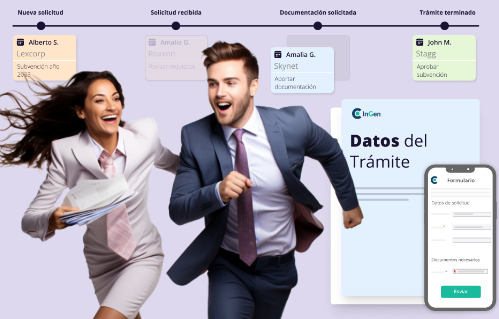
\includegraphics[width=0.7\textwidth]{assets/r2docuotimeline}
    \caption{Captura del homepage de R2 Docuo donde se puede ver el timeline de un trámite}{Fuente: https://www.r2docuo.com/es/expedientes-y-tramites}
    \label{fig:r2docuotimeline}
\end{figure}

Se debe notar que si bien los dos primeros logran la funcionalidad deseada en este proyecto, no permiten la personalización, no son necesariamente software libre y no se pueden introducir en sistemas más grandes de la misma manera que lo haría un paquete de software reutilizable.

\subsection*{Paquetes de software que facilitan la creación de módulos de trámites}

La cantidad de paquetes de software que existen y que se puede considerar que ayudan en el proceso de gestión, control y seguimiento de trámites es abundante, por lo que nos centraremos en aquellas presentes en el ecosistema de Laravel.

El seguimiento de trámites requiere que tengamos guardada la información de todos los pasos de un trámite y los cambios realizados. Además, la naturaleza de los trámites, como se podrá ver en el análisis de la solución, tiene que ver con estados (pasos de un procedimiento administrativo). Es por esto que las siguientes librerías podrían ser utilizadas con un objetivo similar al paquete que se pretende desarrollar en este proyecto:

\begin{itemize}
    \item Laravel Auditing: Permite mantener control sobre los datos en una aplicación y para hacer seguimiento de los cambios realizados en los mismos. Es muy potente y fácil de usar.
    \item Laravel Eloquent State Machines: Máquinas de estado aplicadas sobre los modelos Eloquent (figura \ref{fig:laravelstatemachines}).
    \item Laravel-Permission: Permite asociar usuarios con roles.
\end{itemize}

\begin{figure}[!h]
    \centering
    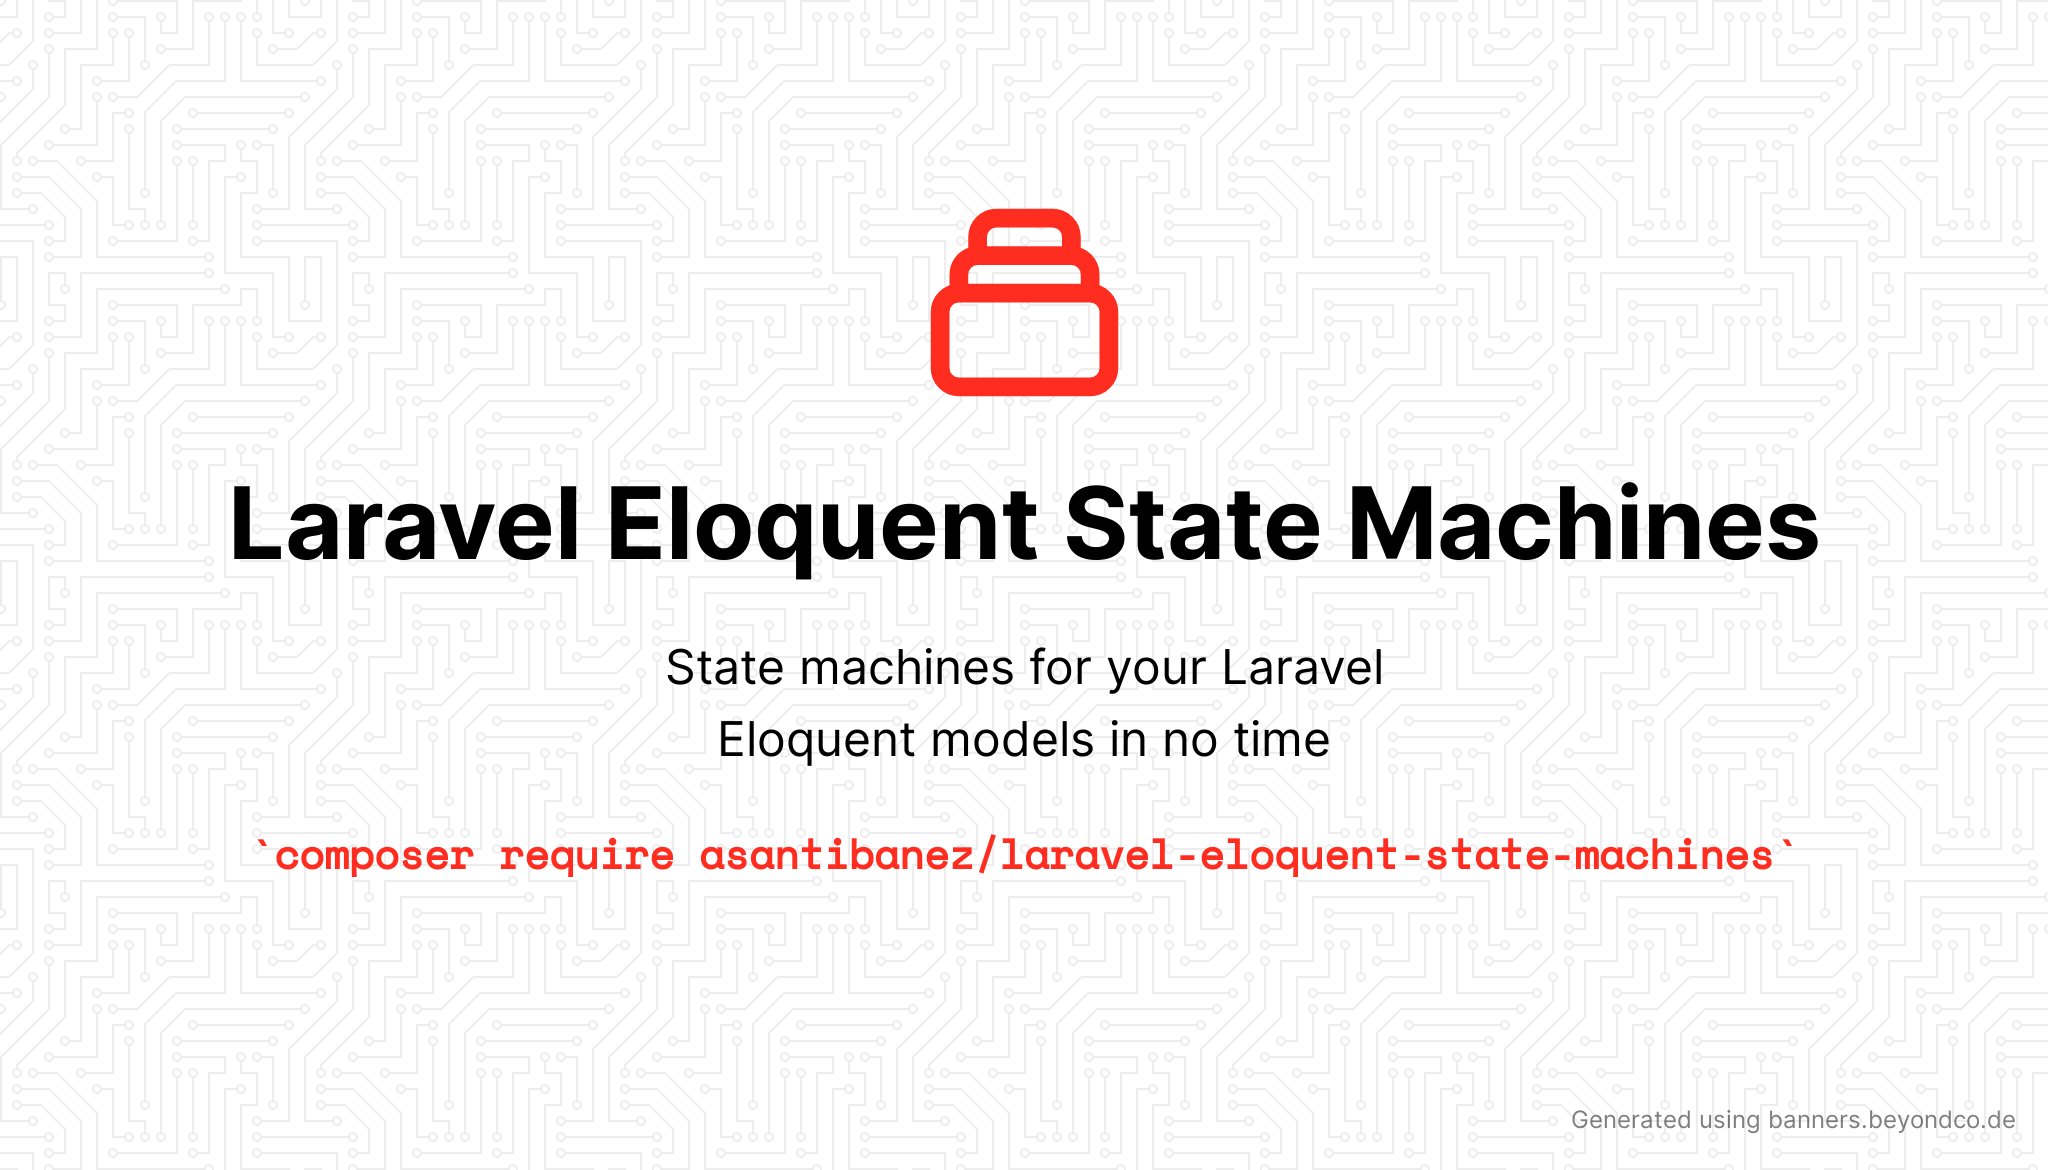
\includegraphics[width=0.7\textwidth]{assets/laravelstatemachines}
    \caption{Paquete de manejo de estados en Laravel}{Fuente: https://github.com/asantibanez/laravel-eloquent-state-machines}
    \label{fig:laravelstatemachines}
\end{figure}

De los tres paquetes anteriores, sin duda el de las máquinas de estados es el que más inspirará este proyecto. La funcionalidad es similar a la que se pretende, pero no es específica a los procesos administrativos y por lo tanto no brinda ciertas herramientas que podrían ser necesarias en los mismos, como el seguimiento, el cual podría ser implementado con la ayuda del segundo paquete mencionado.
